\documentclass[11pt]{article}

\usepackage{url}
\usepackage{color}
\usepackage{float}
\usepackage[format=hang,labelfont=bf,font=small]{caption}
\usepackage{array}
\usepackage{xcolor}
\usepackage{booktabs}
\usepackage[T1]{fontenc}
\usepackage[utf8]{inputenc}
\usepackage[english]{babel}
\usepackage[margin=1in]{geometry}
\usepackage{colortbl}
\usepackage{hyperref}
\usepackage{spreadtab}
\usepackage{longtable}
\usepackage{pdflscape}
\usepackage{subcaption}
\usepackage{amsmath, amsthm, amssymb, amsfonts}
\usepackage{multirow}
\usepackage{graphicx}

\begin{document}

\title{Deep Learning: Homework 2}
\author{Hugo Mantinhas 95592, João Silveira 95597}

\maketitle

\section*{Work Division}

Each member of the group worked together on all the questions in this assignment. For this reason, the workload was divided equally between the two members of the group.

\section*{Question 1}

\subsection*{1.}

The computational complexity of the self-attention layer in a transformer with a single attention head is \(O(L^2D)\), where \(L\) is the sequence length and \(D\) is the hidden size. In order to break down the complexity of this layer, it is important to note that the complexity of matrix multiplication of two matrices of dimensions \(n \times m\) and \(m \times p\) is \(O(nmp)\).

\begin{itemize}
    \item \textbf{Matrix multiplication between \(Q\) and \(K^T\):} This operation has complexity \(O(L^2D)\), since \(Q\) is of size \(L \times D\) and \(K^T\) is of size \(D \times L\).
    \item \textbf{Softmax:} This operation has complexity \(O(L^2)\), since it is applied to a matrix of size \(L \times L\).
    \item \textbf{Matrix multiplication between \(Softmax(QK^T)\) and \(V\):} This operation has complexity \(O(L^2D)\), since the result of the previous operation is of size \(L \times L\) and \(V\) is of size \(L \times D\).
\end{itemize}

Therefore, the overall complexity of the self-attention layer is given by: 

\[
O(L^2D) + O(L^2) + O(L^2D) = O(L^2D)
\]

This can be problematic for long sequences due to the quadratic dependence on the sequence length \(L\). This makes this self-attention layer computationally expensive and increasingly impractical for very long sequences.

\subsection*{2.}

The third expansion for the McLaurin series for approximating the exponential function $e^z$ is expressed as follows:

\begin{equation}
e^z \approx 1 + z + \frac{z^2}{2}
\label{q1:2-mclaurin}
\end{equation}

Applying this approximation to \(e^{q^Tk}\), where \(q, k \in \mathbb{R}^D\), yields:

\[
e^{q^Tk} \approx 1 + q^Tk + \frac{(q^Tk)^2}{2}
\]

Now, notice the that following is true, according to the multinomial theorem~\footnote{\url{https://en.wikipedia.org/wiki/Multinomial_theorem}}:

\[
(\sum_{i}{a_i})^2 = \sum_{i}{a_i^2} + 2 \sum_{i < j}{a_ia_j}
\]

Applying this theorem, we can expand \((q^T k)^2\) as follows:

\[
(q^Tk)^2 = \sum_{i=1}^{D}{(q_i k_i)}^2 + 2 \sum_{i < j}^{D}{q_i k_i q_j k_j}
\]

Which, when reorganized to make the feature map derivation more clear, looks as follows:

\[
(q^Tk)^2 = \sum_{i=1}^{D}{q_i^2 k_i^2} + 2 \sum_{i < j}^{D}{q_i q_j k_i k_j}
\]

Thus, we get the final approximation for \(e^{q^Tk}\):

\[
e^{q^Tk} \approx 1 + \sum_{i=1}^{D}{q_i k_i} + \frac{\sum_{i=1}^{D}{q_i^2 k_i^2}}{2} + \sum_{i < j}^{D}{q_i q_j k_i k_j}
\]

Finally, to capture this approximation through a feature map \(\phi: \mathbb{R}^D \rightarrow \mathbb{R}^M\), we define:

\[
\phi(q) = 
\begin{bmatrix} 
1 \\ 

q_1 \\ 
\vdots \\ 
q_D \\

\frac{1}{\sqrt{2}}q_1^2 \\
\vdots \\
\frac{1}{\sqrt{2}}q_D^2 \\

q_1q_2 \\
\vdots \\
q_{D-1}q_D
\end{bmatrix}
\]

Regarding the dimensionality, \(M\), we can invoke the multinomial theorem result for the number of coefficients, to calculate the number of coefficients of equation \ref{q1:2-mclaurin}.

\[
M = 1 + D + \binom{2 + D - 1}{D - 1} = 1 + D + \frac{(D+1)D}{2}
\]

Lastly, for the scenario where $K \geq 3$ terms are employed in the McLaurin series expansion, the dimensionality $M$ can be generalized. Similarly as above, we can also employ the multinomial theorem for values bigger than 2:

\[
M = 1 + D + \sum_{J=2}^{K}{\binom{J + D - 1}{D - 1}}
\]

\section*{Question 2}

\subsection*{1.}

The best configuration has a learning rate of $0.01$. It provided the best results in terms of final test accuracy: $0.8488$.

\begin{figure}[H]
    \hspace{0.025\linewidth}
    \begin{subfigure}{0.45\linewidth}
        \centering
        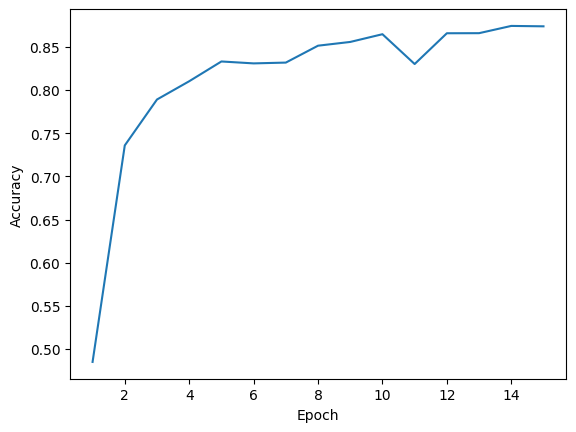
\includegraphics[width=\linewidth]{../data/q2/1/0.01.acc.png}
        \caption{Validation accuracies for learning rate of 0.01 with max pooling}
    \end{subfigure}
    \hspace{0.05\linewidth}
    \begin{subfigure}{0.45\linewidth}
        \centering
        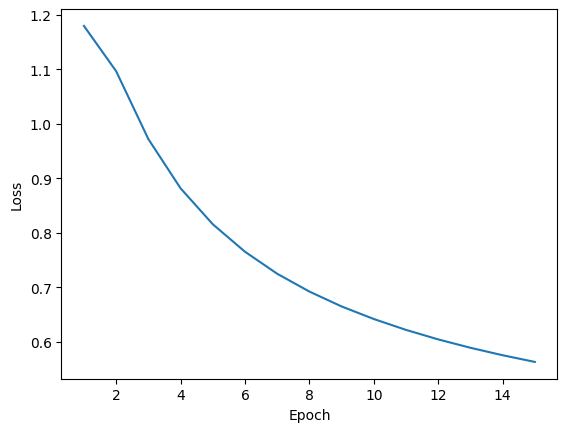
\includegraphics[width=\linewidth]{../data/q2/1/0.01.loss.png}
        \caption{Losses as a function of the number of epochs for learning rate of 0.01 with max pooling}
    \end{subfigure}
\end{figure}

\subsection*{2.}

Using the optimal hyper-parameters found in the previous question, that is, with the learning rate of $0.01$, we trained the model for 15 epochs and obtained a final test accuracy of $0.8299$.

\begin{figure}[H]
    \hspace{0.025\linewidth}
    \begin{subfigure}{0.45\linewidth}
        \centering
        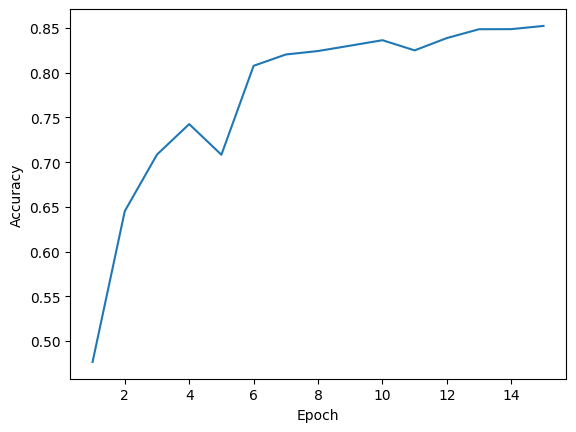
\includegraphics[width=\linewidth]{../data/q2/2/0.01.acc.png}
        \caption{Validation accuracies for learning rate of 0.01 without max pooling}
    \end{subfigure}
    \hspace{0.05\linewidth}
    \begin{subfigure}{0.45\linewidth}
        \centering
        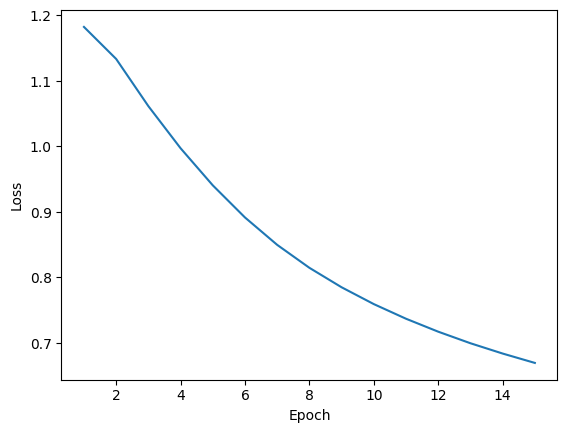
\includegraphics[width=\linewidth]{../data/q2/2/0.01.loss.png}
        \caption{Losses for learning rate of 0.01 without max pooling}
    \end{subfigure}
\end{figure}

\subsection*{3.}

The number of trainable parameters ($225618$) remains unchanged between both CNNs. Consequently, for the training stage, both CNNs have the same expressivity to adjust to data. The more significant difference comes from the application, or absence, of the max pooling layer. The max pooling layer provides many benefits that can justify the model's higher performance. Max pooling will select the highest value of each region and store it, discarding the remaining values. This will discard a lot of potentially less important information and noise, and only keep the highest values, which carry meaning in our network. Max pooling will, inevitably, reduce the spatial dimensions of the input data, however, by definition of the max function, it will always preserve the highest value across pools. This can provide the model translation, rotation, and scale invariance, an important property when classifying images.

\section*{Question 3}

\end{document}